% !TEX root = paper.tex

\documentclass[11pt,letterpaper]{article}

% Packages
\usepackage{packages}
\addbibresource{sources.bib}

% Document Settings
\geometry{margin=1in}
\setlength{\parskip}{1ex}
\setlength{\parindent}{0pt}

\pagestyle{fancy}
\lhead{Väinö-verneri Kauppila} % controls the left corner of the header
\chead{} % controls the center of the header
\rhead{} % controls the right corner of the header
\lfoot{} % controls the left corner of the footer
\cfoot{} % controls the center of the footer
\rfoot{Page~\thepage} % controls the right corner of the footer
\renewcommand{\headrulewidth}{0.4pt}
\renewcommand{\footrulewidth}{0.4pt}

% =========================================
%             DOCUMENT
% =========================================

\begin{document}
%\doublespacing % Double spacing throughout the document


% =========================
%      TITLE PAGE
% =========================

% Suppresses headers, footers, and page numbers on title page
\begin{titlepage}
    \begin{center}
        \vspace*{4cm}
        Geography\\
        Internal Assessment \\
        \vspace{1cm}
        How does environmental quality, determined by the severity of pollution and the availability of green spaces, differ between a tourist-catering area of Paris versus a residential area? \\
        \vspace{1cm}
        \textit{Väinö-verneri Kauppila} \\
        May 2021 \\
        \vspace{4cm}
        Word count: TBD \\
        \vfill
        \vspace{0.1cm}
    \end{center}
\end{titlepage}

% =========================
%      DOCUMENT BODY
% =========================

\pagenumbering{roman}

\begin{center}
    \pdfbookmark{\contentsname}{Contents}
    \tableofcontents
    \vspace{1in}

\end{center}


% TODO: Add hyper-references to links
% TODO: Improve listings' styling
% TODO: Add links to Contents entries

\newpage

\pagenumbering{arabic}

\section{Introduction}

\subsection{Fieldwork question}

How does environmental quality, determined by the severity of pollution and the availability of green spaces, differ between a touristic area of Paris and a residential area?

The fieldwork for our paper was conducted in Paris, one of the largest and most well known cities in the world. The city itself is arranged in a manner such that 20 districts, known locally as \textit{arrondissements}, are placed in a spiral in the city. It is globally known for its high number of tourists per year, equating to around 35 million tourists in the year 2019 alone. \footcite{statista_department_27_2020} Many of them come to visit the world-renowned Eiffel Tower, located in the VII\textsuperscript{th} \textit{arrondissement}. \footcite{condor_ferries} To add, Paris is home to 2.2 million people, who mostly live in the outer residential areas, from the XI\textsuperscript{th} to the XX\textsuperscript{th} \textit{arrondissements}.

\begin{figure}[h!]
    \centering
    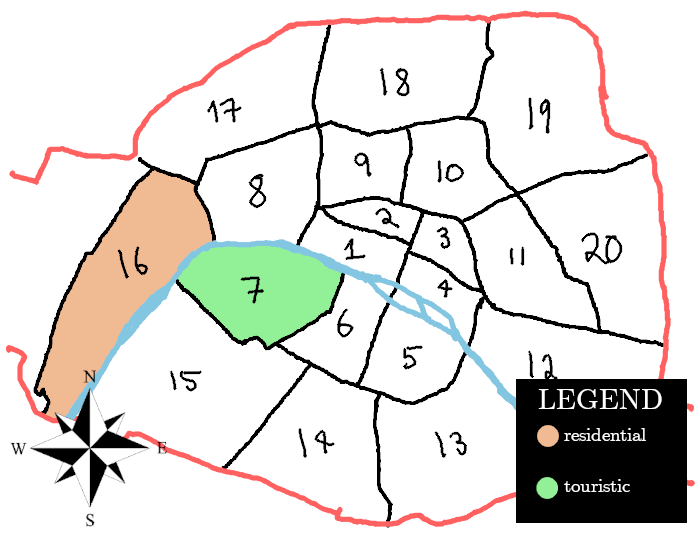
\includegraphics[width=0.7\linewidth]{arrts.png}
    \caption{A map of Paris \textit{arrondissements}, drawn by hand.}
\end{figure}



\subsection{Hypotheses}

\begin{enumerate}
    \item According to the Global Development Goals of the UN, 90\% of urban areas in the world had polluted air in 2016. \footcite{sdg_report_2020} Paris was among these countries that didn't satisfy WHO's air quality minimum \footcite{ambient_outdoor_air_pollution_2018} of 2018, with on average a 50\% higher than normal pollution density. In addition, the areas of tourism in Paris are, as seen in Figure 2, higher in pollution than residential areas. However, a counterargument to this could be that despite a higher concentration of people, tourist areas in Paris do not suffer as much from high traffic conditions from things such as typical morning rush hours, and tourists preferably using public transport or bikes.

    \item As there are more people moving about in residential areas, for example in cars for the morning commute or at noon for lunch, it can logically be theorized that noise pollution, which is obviously a function of the amount of people, would be higher in these places. Today it is estimated that an average noise level of $60dB$ can be found in residential areas, according to the comprehensive Bruitparif government-sponsored report. \footcite{bruitparif} This value largely surpasses the WHO's safe level of $53dB$. \footcite{who_noise_guidelines} 
    
    \item The Parisian mayor, Anne Hidalgo included the betterment of the environment in her campaign. The mayor has promised to make so-called "green spaces" no further than 200 meters to any person,\footcite{anne_hidalgo_2020} and as such, it should be hypothesized that green spaces, which include parks, agglomerations of trees, shall be distributed evenly with no difference between residential and touristic areas. The mayor emphasized on "urban forests" --- places where residents and tourists alike could enjoy the company of trees while walking along the city streets. 
\end{enumerate}


\begin{figure}[h!]
    \begin{minipage}{\textwidth}
    \centering
    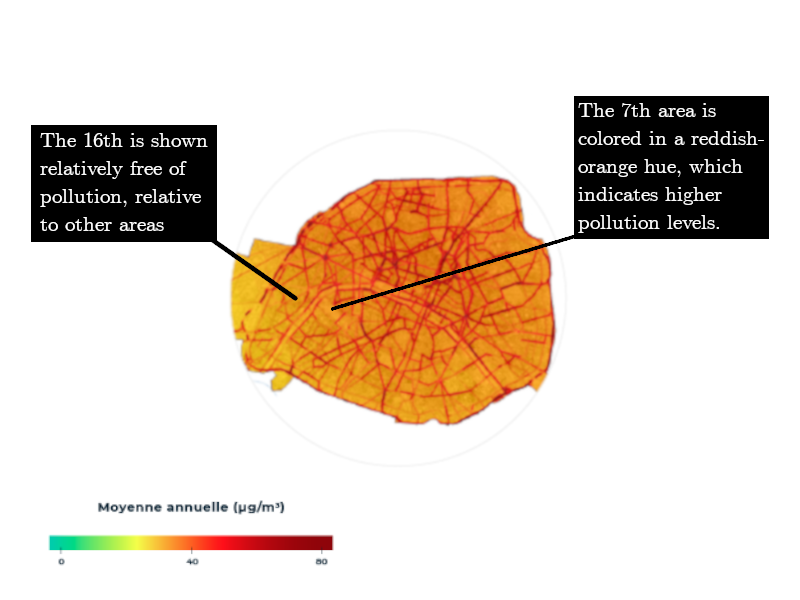
\includegraphics[width=0.7\linewidth]{no2_map.png}
    \caption{A map of Paris NO2 levels in 2018, as reported by AirParif, on the official Paris website \protect\footcite{paris_air_qual}}
    \end{minipage}
\end{figure}



\section{Method}


For our investigation, the topic in question is the environmental quality. We shall compare the environmental quality of two areas, one meant as a residential one and one with a heavy tourist presence. To best represent these areas, we have chosen the XVIe and the VIIe, justifiable as the XVIe is home to many housing complexes and fosters facilities aimed at catering to the residents whereas the VIIe sees many tourists as it is home to the famed Eiffel Tower and the Seine river, prime tourist attractions of Paris.

\subsection{Study site choices}

We chose 10 sites in total to study, shown below in Figures 3, 4. 

\begin{figure}[H]
    \begin{minipage}{\textwidth}
    \centering
    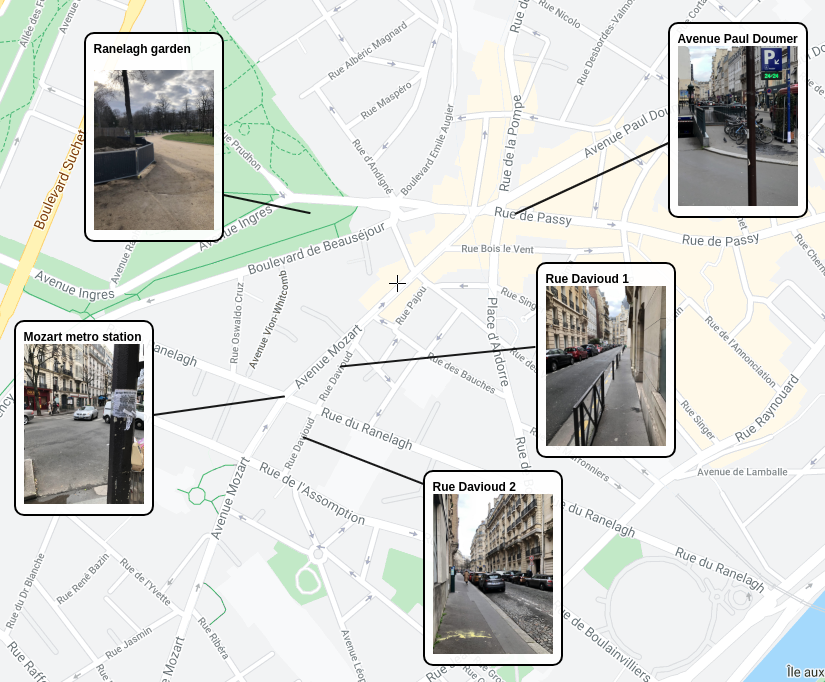
\includegraphics[width=0.7\linewidth]{16esites.png}
    \caption{Map of sites chosen for the residential area, the XVI\textsuperscript{th} \textit{arrondissement}. Map base layer courtesy of Google Maps, pictures seen are taken on a mobile phone.}
    \end{minipage}
\end{figure}

\begin{figure}[H]
    \begin{minipage}{\textwidth}
    \centering
    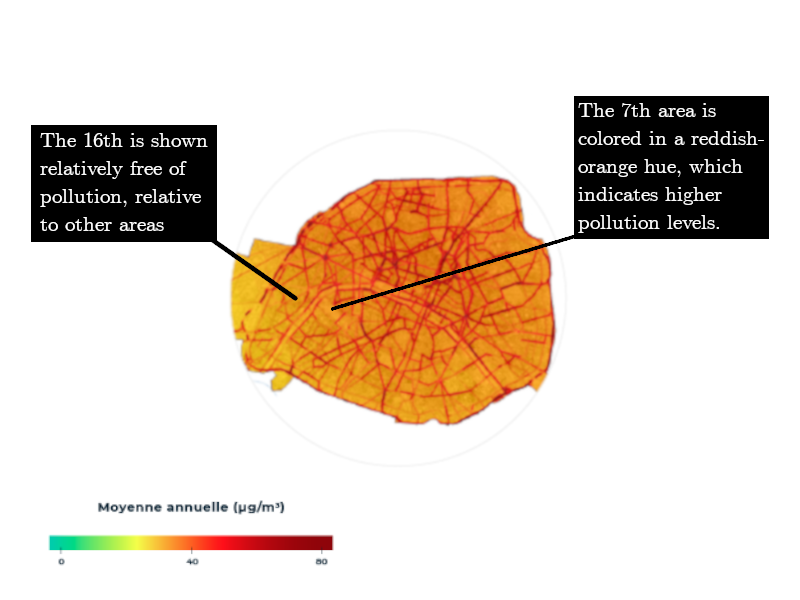
\includegraphics[width=0.7\linewidth]{no2_map.png}
    \caption{Map of sites chosen for the residential area, the XVI\textsuperscript{th} \textit{arrondissement}. Map base layer courtesy of Google Maps, pictures seen are taken on a mobile phone.}
    \end{minipage}
\end{figure}

\subsection{Sampling choices}

The method we will be using to select the sites from where we will take the Bipolar survey is Stratified which means that we are choosing the sites ourselves. The reason we chose this is to make sure that we got a good variety of sites that would give a good idea of the general environmental quality of that area, but also to avoid the selection of residential areas, which do in fact exist in the VIIe, which would happen if we chose the random sampling method. This stratified sampling approach would best represent the targeted area and yield meaningful data on tourist-heavy sites.

The sampling method we used to select our sites is the stratified method. The reason for this choice is that we get a


\section{Analysis}

Lorem

\subsection{Environmental and cultural sustainability}
Lorem ipsum dolor sit amet

\subsection{Economic sustainability}
Lorem ipsum dolor sit amet

\section{Conclusion}

Lorem ipsum dolor si amet

\newpage
\pagenumbering{roman}


\section*{Notes}
\label{sec:notes}
\addcontentsline{toc}{section}{\nameref{sec:notes}}

This paper is written with the aid of the typesetting software \LaTeX. On a PDF viewer, the sections in the table of contents can be clicked to access that section.

\printbibliography

\appendix
\section{Appendix}
\label{app}

\subsection{Appendix Test}
\label{app:test}


\end{document}